\section{Results}
Cuts flow: 7143 $\rightarrow$ 6873 ($z$) $\rightarrow$ 2465 (mask). Cosmo SNe \NCosmo: void \NVoidCosmo, wall \NWallCosmo\ (\NShellCosmo\ shell, \NOutCosmo\ outside; Table~\ref{tab:counts}). Observed void fraction $\NVoidCosmo/\NCosmo=0.074$ versus randoms $0.173$: apparent (uncorrected) void/wall ratios \RRall\ all, \RRia\ Ia-only (\NIaVoid/\NIaWall), \RRcc\ CC-only (\NCCVoid/\NCCWall); Poisson+Monte Carlo rel.\ err $0.08$--$0.18$. No efficiency or host-mass correction applied, so these are apparent deficits in a flux-limited sample, not intrinsic rates. Table~\ref{tab:counts} sums exactly; shell/outside rows are tabulated, not dropped. Void holds \NIaVoid\ SN Ia (subtype audit pending TNS). Volume slice $z\le0.06$: 1270 SNe total, 71 void (44 Ia). Threshold grid (SNe): 0.6:59, 0.7:103, 0.8:176, 0.9:288, 1.0:435, 1.1:609. Redshift stability $z_{\min}$ 0.01:176, 0.02:171, 0.025:168, 0.03:164 void. Void median $z$ 0.069 versus wall 0.055 confirms Malmquist gradient.
\begin{table}
\caption{Masked sample composition. Wall means finite $1.0<r/R_{\max}<\infty$; Outside is $r/R_{\max}=\infty$ (no void within $1.2\max R_{\max}$). Cosmo-grade excludes 91T/91bg/pec/Iax/CSM/SC.}
\label{tab:counts}
{\small\setlength{\tabcolsep}{3pt}
\begin{tabular}{lrrrrr}
\hline
Sample & Total & Void & Shell & Wall & Outside \\
\hline
All-types & 2465 & 183 & 271 & 1950 & 61 \\
Cosmo-grade & 2381 & 176 & 262 & 1883 & 60 \\
Normal Ia & 1785 & 141 & -- & 1393 & -- \\
CC & 582 & 35 & -- & 479 & -- \\
\hline
\end{tabular}}
\end{table}

\begin{figure}
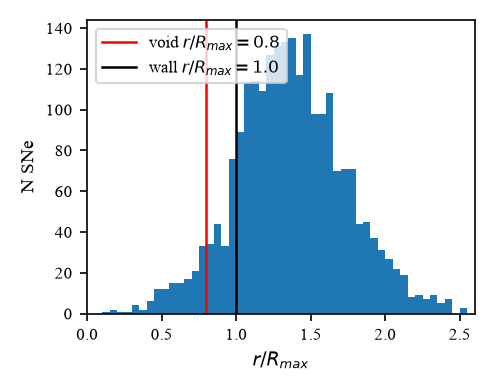
\includegraphics[width=\columnwidth]{figures/rRv_hist_v2.png}
\caption{$r/R_{\max}$ (52 bins, $0$--$2.6$) for $N=\NCosmo$ cosmology-grade SNe (void $r/R_{\max}<0.8$, $N=\NVoidCosmo$; wall $>1.0$). Red/black lines mark the analysis thresholds.}
\label{fig:rrv}
\end{figure}

\begin{figure}
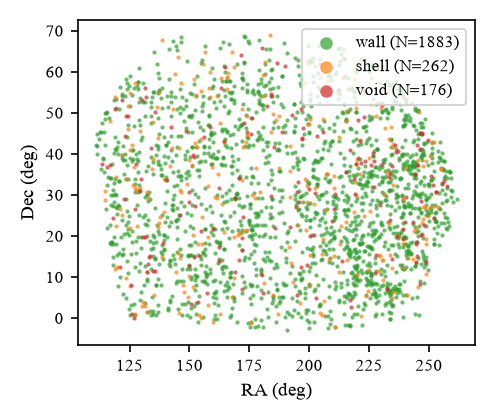
\includegraphics[width=\columnwidth]{../plots/footprint_v2.png}
\caption{Masked RA--Dec distribution colour-coded by environment.}
\label{fig:foot}
\end{figure}

FRB error budget (Cat1): per-sightline $\sigma_{\rm tot}\sim150$--$200\,{\rm pc\,cm^{-3}}$ (IGM 80--120, host 80--150, Milky Way residual 20--40 with NE2001$-$YMW16 median $-3.3$, std $37.5$, p90 $68.1$, halo 20). Void signal $\sim10$--$30$. A $\delta{\rm DM}<50$ limit at 95 per cent needs $N_{\rm void}\gtrsim36$ ($\sim200$ localised total); unlocalised $z<0.114$ needs $\sim900$ void sightlines, have $\sim30$--$50$.
